\subsection{Interconexión de clusters}\label{s:interconexion}

Para determinar qué es lo que causa la división en el segundo pico de la 
RDF$_{Si-Li}$ se realizó un análisis similar al reportado por Ding \textit{et al.}
~\cite{ding2015}. Estos autores analizaron la correlación en la distancia de a
pares de los segundos vecinos más cercanos en términos de las conexiones entre
clusters, definiendo un poliedro de coordinación alrededor del átomo central 
considerado para la RDF y sus segundos vecinos. El número de átomos compartidos
entre estos dos poliedros de coordinación enlazados fueron utilizados para 
establecer categorías y analizar sus contribuciones a la RDF. Estas categorías
dependen del hecho de que los poliedros comparten un vértice (1 átomo), una 
arista (2 átomos), una cara de los poliedros (3 átomos) o cuadriláteros 
distorsionados o tetraedros aplastados (4 átomos). De una forma similar a este 
trabajo, se deconvolucionó el segundo pico de la RDF calculando la RDF parcial 
de distintas categorías, donde cada categoría se define por el número de átomos de
Li que interconectan un átomo de Si con su segundo vecino de Li. El comportamiento
detallado se presenta en la figura \ref{fig:interconexiones}. Puede afirmarse a 
grandes rasgos que para concentraciones bajas de Li en las aleaciones, hay una 
predominancia de segundos vecinos de Li que tienen una o ninguna interconexión 
con los vecinos de Li de la primera esfera de coordinación Si-Li. Para $x > 1.0$
la contribución del segundo vecino de Li interconectado con dos o más átomos de 
Li de la primera esfera de coordinación Si-Li comienza a ser predominante y la
contribución de los átomos de Li sin conectarse empieza a decaer. Para $x > 3.0$,
la contribución del primer pico del segundo vecino de Li interconectado dos o
tres veces se vuelve relevante mientras que aparecen contribuciones de cuatro o
más interconexiones.
\begin{figure}[th]
    \centering
    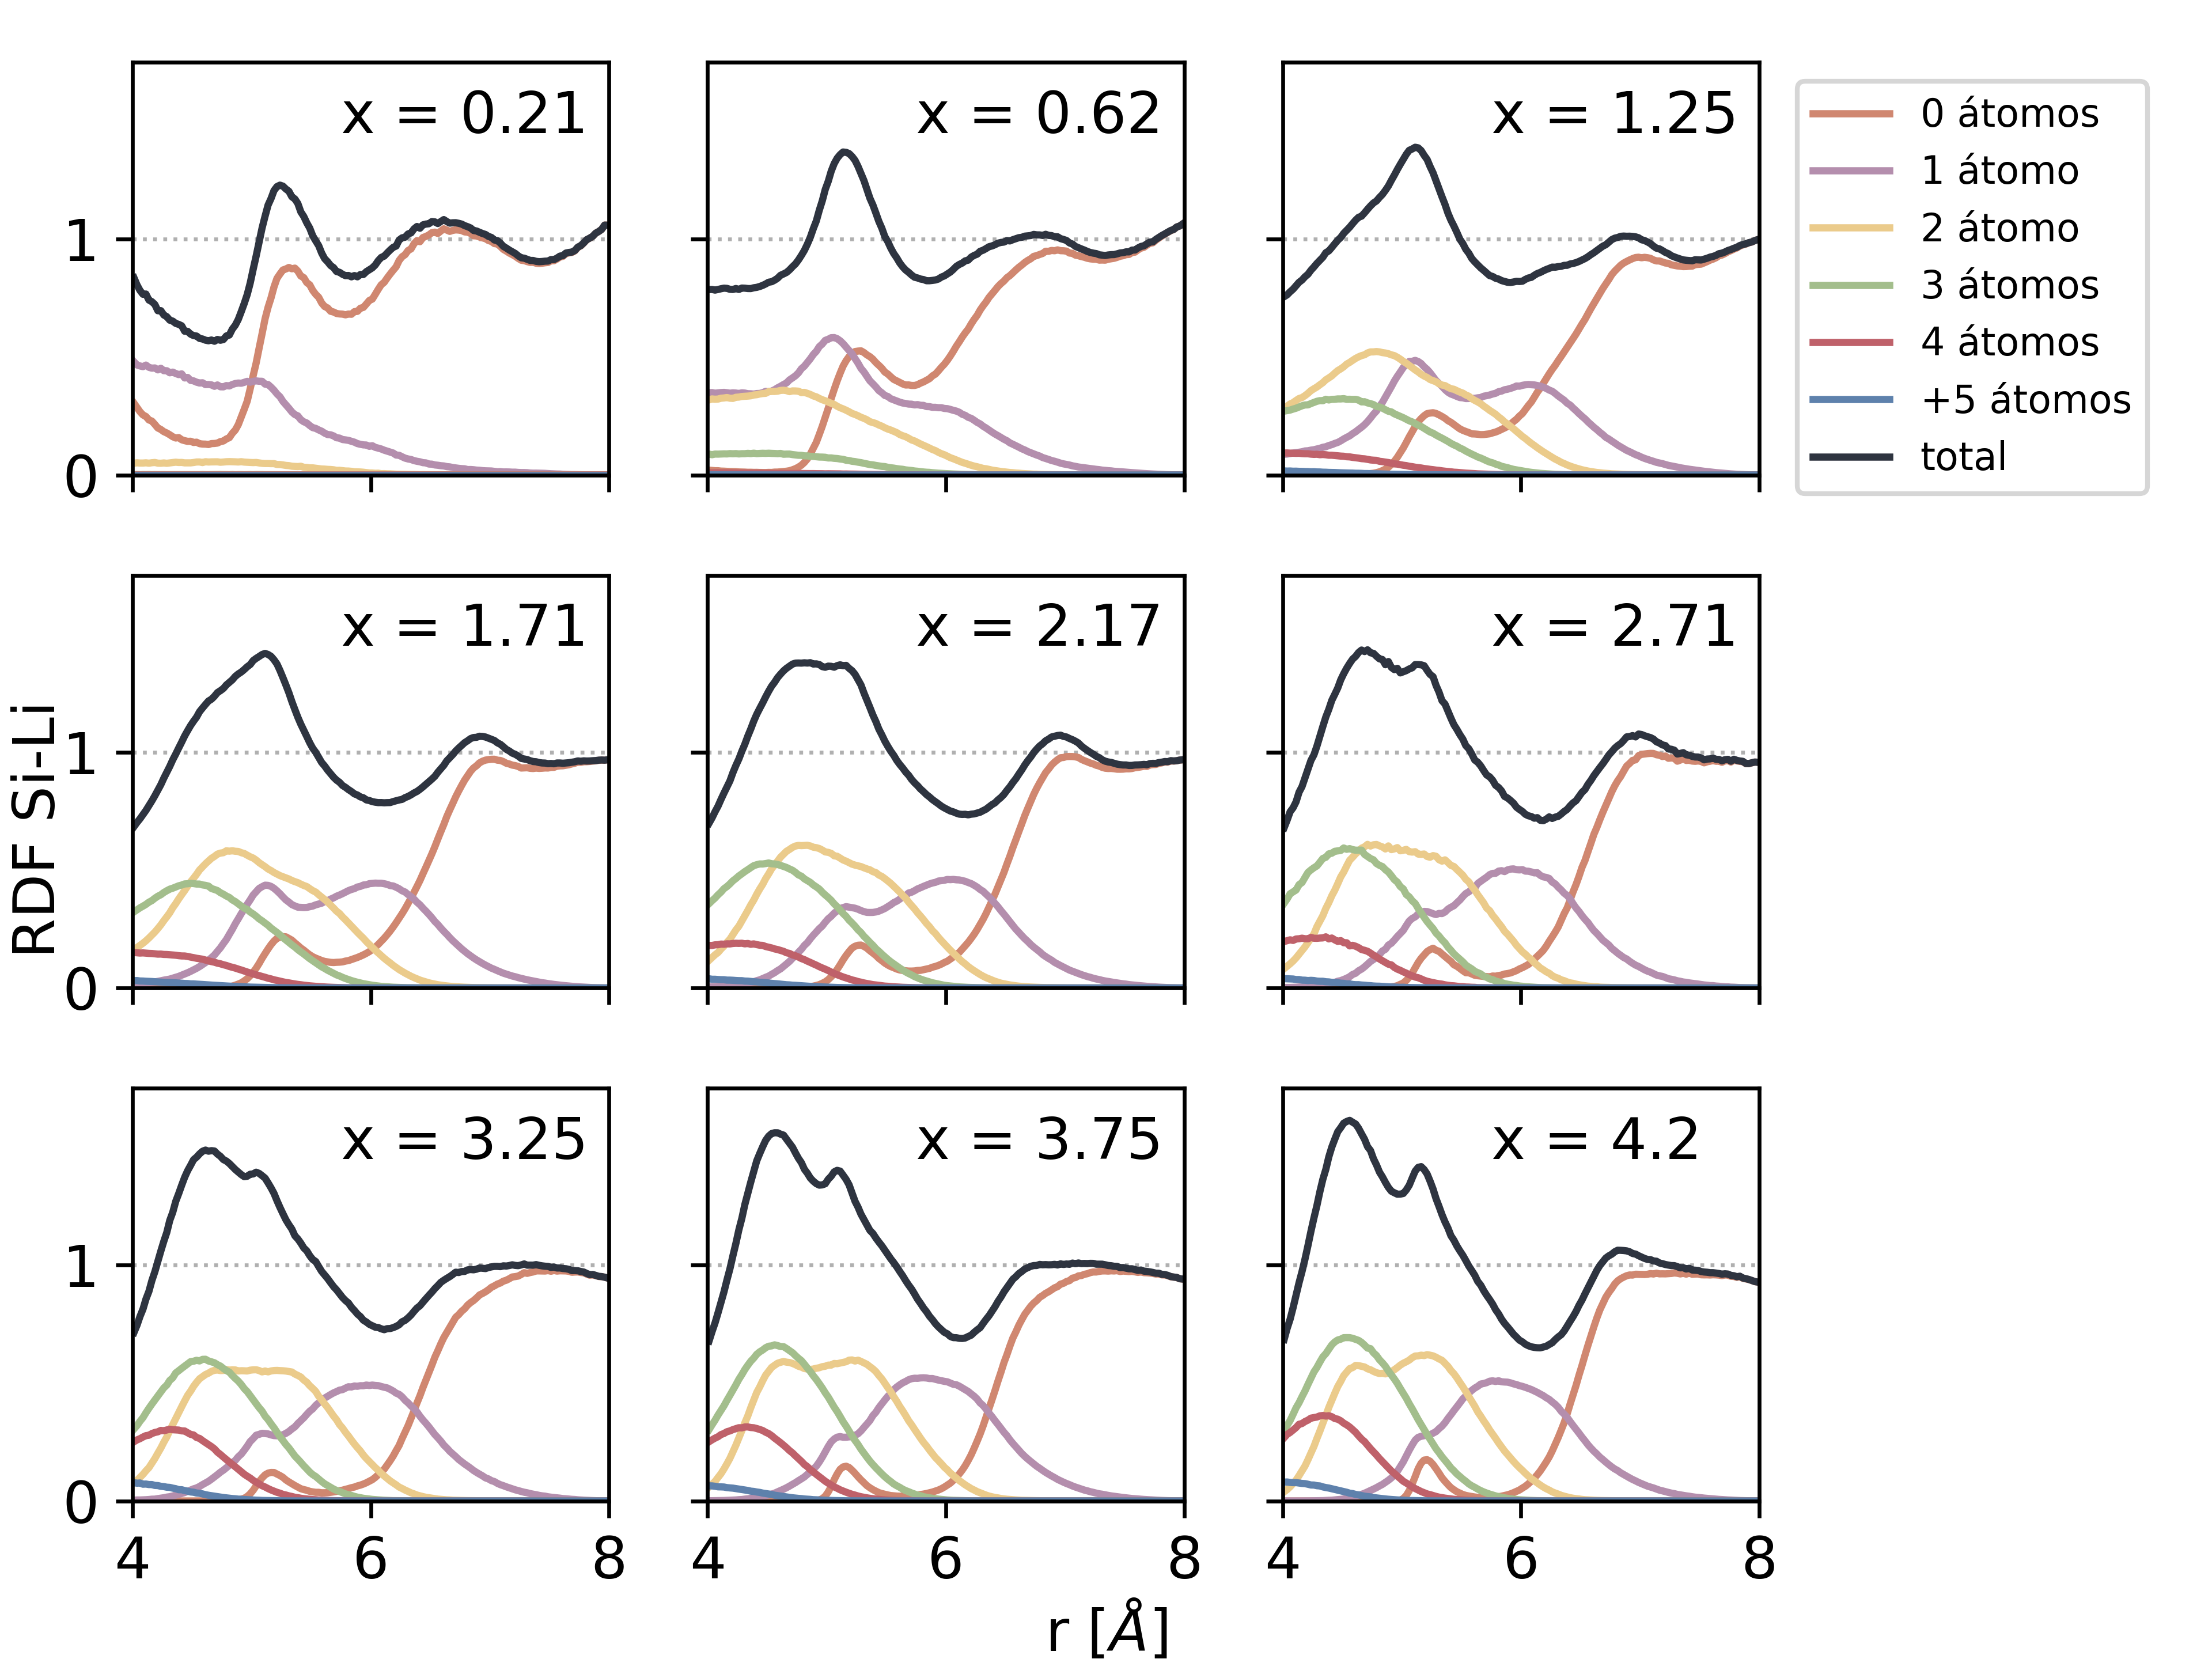
\includegraphics[width=\textwidth]{caracterizacion/resultados/interconexion/interconexiones.png}
    \caption{Interconexiones de los segundos vecinos más cercanos de Li con un 
    átomo central de Si para cada valor de $x$ en Li$_x$Si considerado. El número 
    de primeros vecinos más cercanos que conectan a los segundos vecinos más 
    cercanos con el átomo central de Si se indica en el recuadro de las figuras. 
    Además de la RDF$_{Si-Li}$ total, se grafica cada una de las contribuciones 
    de los diferentes tipos de interconexiones posibles.}
    \label{fig:interconexiones}
\end{figure}

Mientras que el comportamiento presentado en la figura \ref{fig:interconexiones}
es más bien complejo, pueden establecerse tendencias generales que ayudan a 
entender mejor que es lo que sucede. Si se divide la RDF$_{Si-Li}$ en dos 
contribuciones de segundos vecinos, la primera de ellas, que se encuentra a una
distancia entre 4.0 \AA\ y 5.0 \AA, se puede atribuir a los átomos que tienen dos 
o más interconexiones de Li, mientras que la segunda de ellas, entre 5.0 \AA\ y
5.6 \AA, se corresponde con los átomos que tiene una o ninguna interconexión de 
Li. Utilizando esta clasificación, se muestra en la figura 
\ref{fig:interconexiones-areas} la fracción del área que representa cada una de
estas categorías en función de la concentración de litio.
\begin{figure}[th]
    \centering
    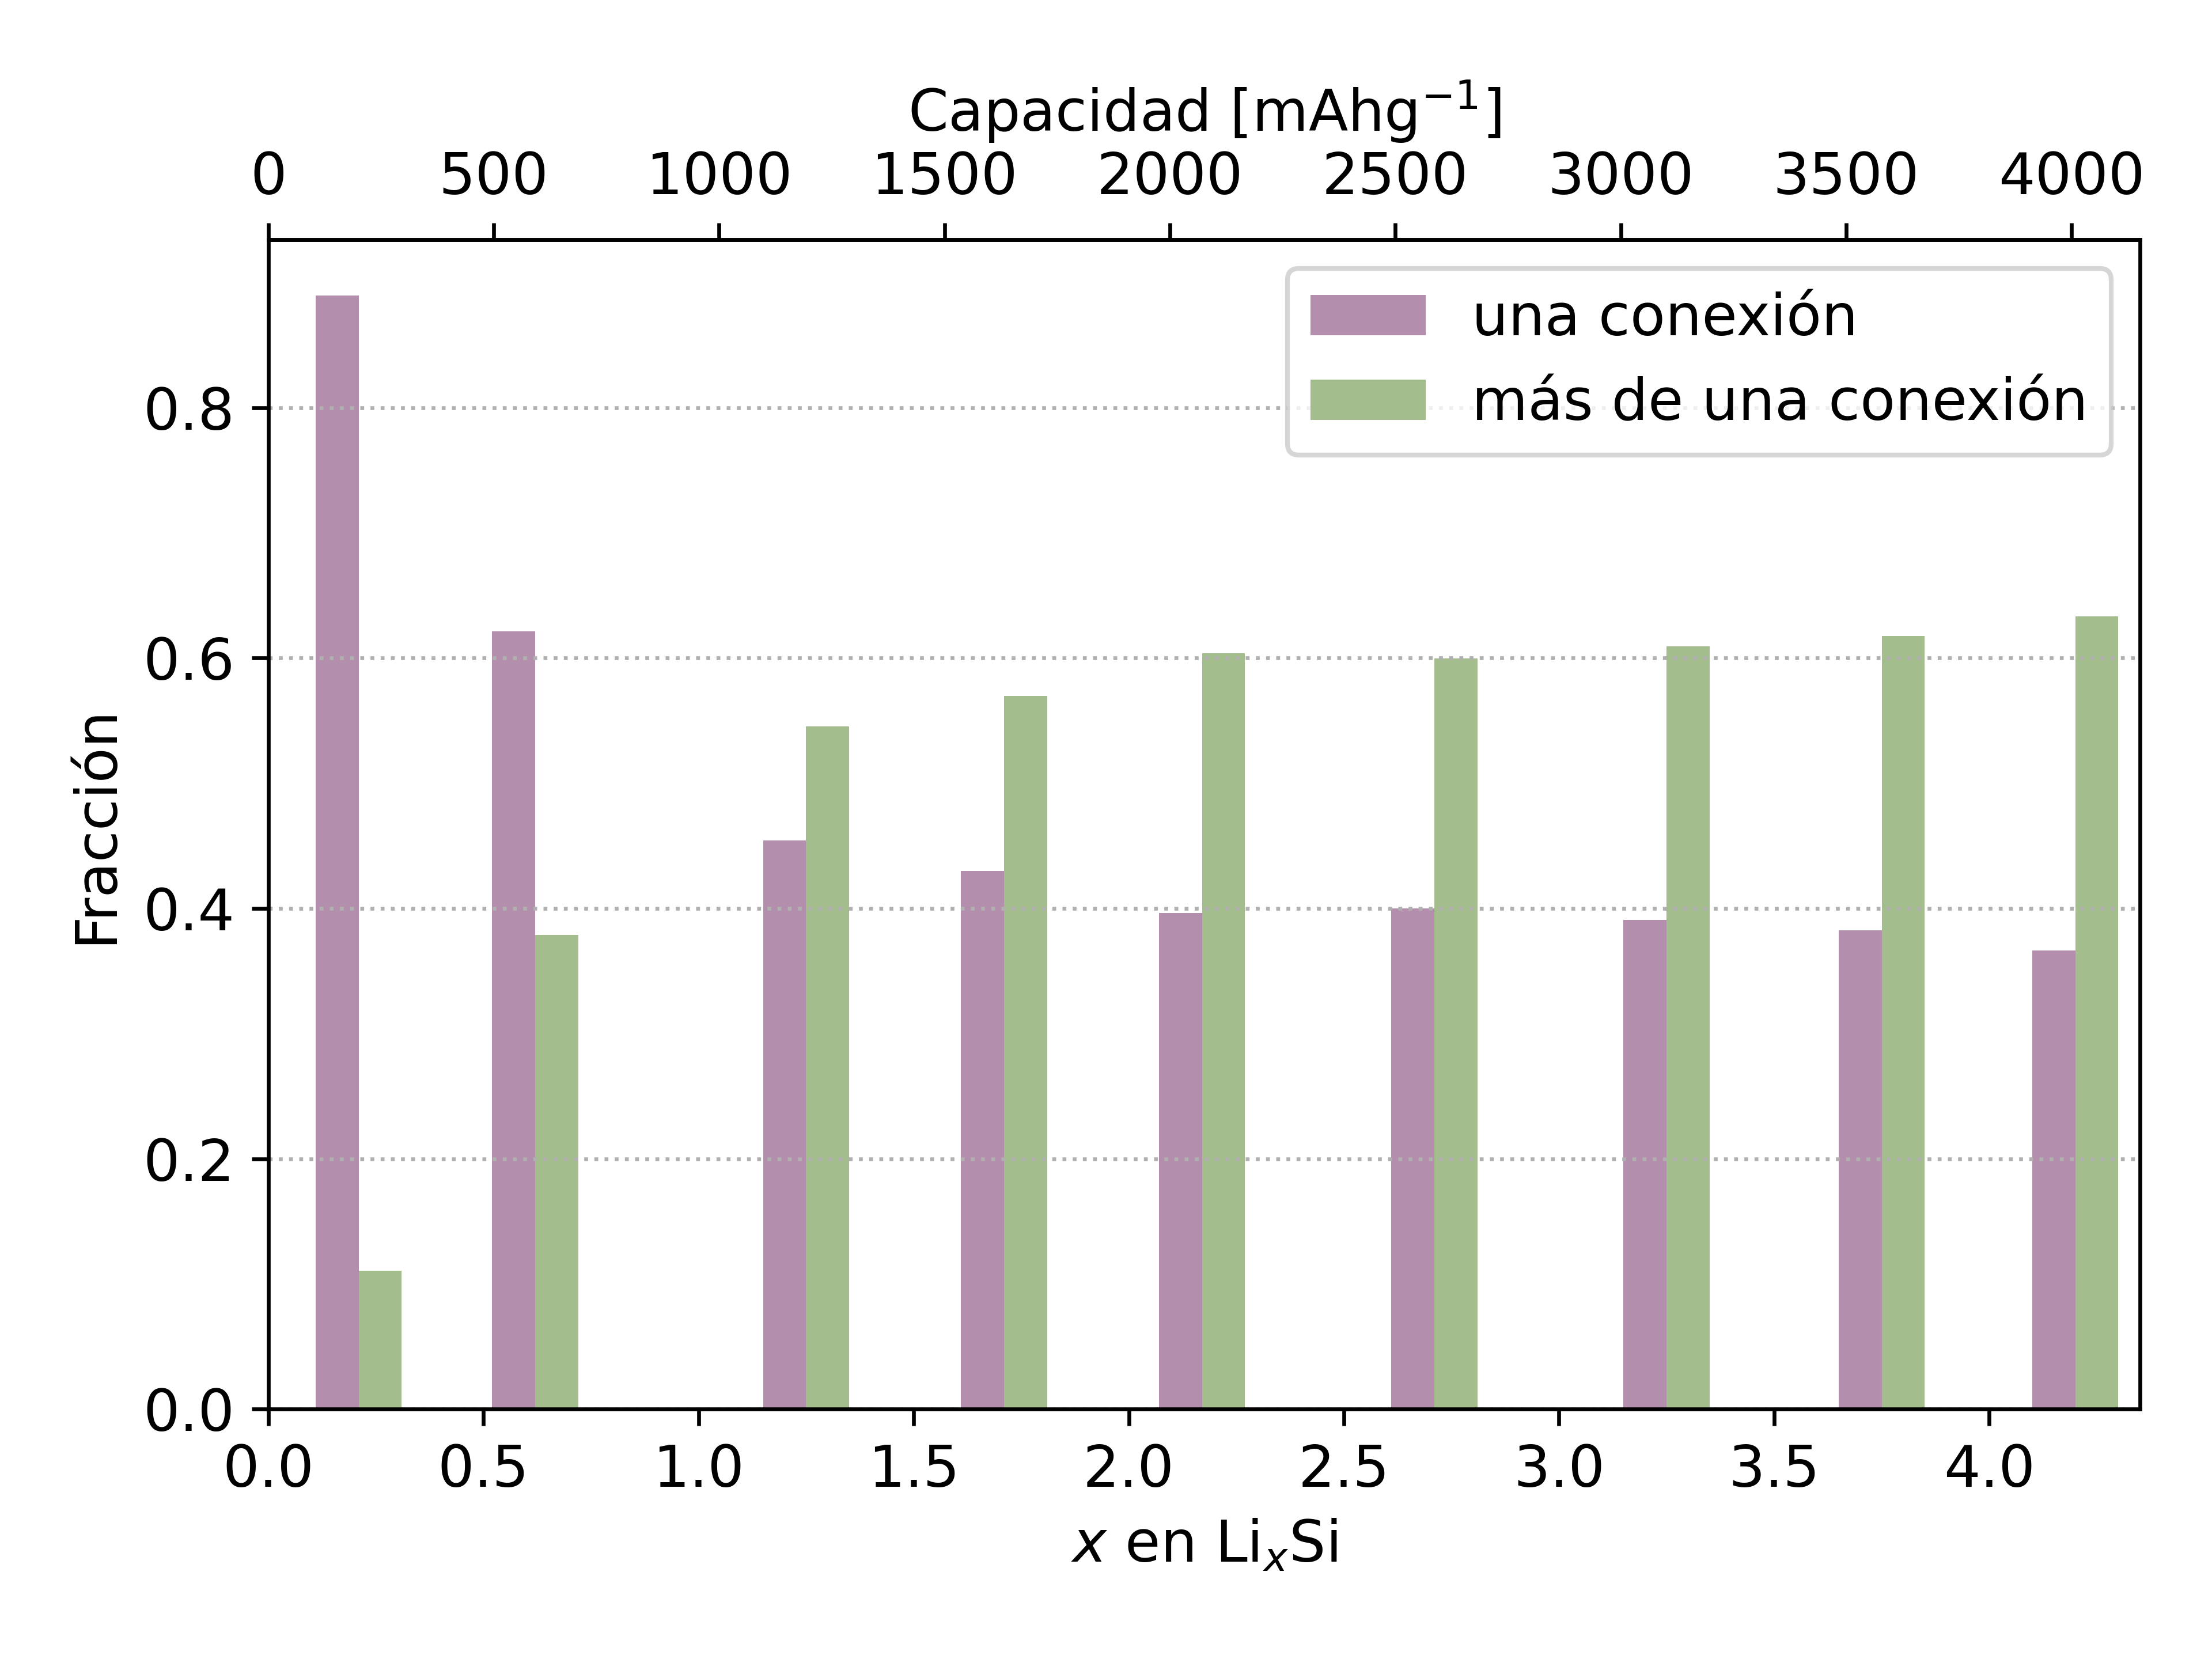
\includegraphics[width=0.8\textwidth]{caracterizacion/resultados/interconexion/interconexiones-areas.png}
    \caption{Evolución con la concentración de la fracción que representa cada
    categoría de interconexiones de Li al área total del segundo pico de la 
    RDF$_{Si-Li}$.}
    \label{fig:interconexiones-areas}
\end{figure}
